\begin{explanationbox}
\textbf{\textcolor{CExplanation}{先看图：同一条焦点弦的两端点，不必关于 $x$ 轴对称}}\par\smallskip
% 保留原文件原样引用位置；原始被引用图未随附件提供，包内补齐此依赖。
\begin{minipage}{\linewidth}
\begin{center}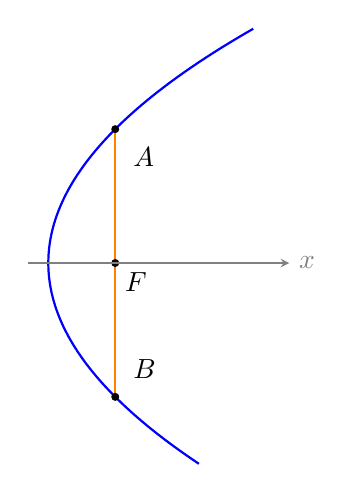
\begin{tikzpicture}[scale=0.85,>=stealth]
\draw[blue,thick,domain=-3:3.5,samples=90] plot ({\x*\x/4},\x);\draw[orange,thick] (1,-2)--(1,2);\fill (1,0) circle (1.7pt) node[below right] {$F$};\fill (1,2) circle (1.7pt) node[below right=3pt] {$A$};\fill (1,-2) circle (1.7pt) node[above right=3pt] {$B$};\draw[->,gray] (-.3,0)--(3.6,0) node[right] {$x$};
\end{tikzpicture}
\end{center}
\end{minipage}
\par\smallskip
图中 $p=2$，取过焦点 $F(1,0)$ 的直线 $x=\frac34y+1$，
得到 $A(4,4)$、$B(\frac14,-1)$：
\[
 4\times\frac14=1=\frac{p^2}{4},\qquad
 4\times(-1)=-4=-p^2.
\]
注意 $A,B$ \textbf{并不关于 $x$ 轴对称}，却仍保持定值。

\medskip
\textbf{\textcolor{CExplanation}{第一层：用最熟悉的图形观察}}\par\smallskip
焦点横坐标是 $\frac p2$。先看最简单的\textbf{通径}：
$x=\frac p2$，于是 $y=\pm p$，两端点为
\[
 \left(\frac p2,p\right),\quad \left(\frac p2,-p\right).
\]
因此纵坐标一正一负，积为 $-p^2$；横坐标都等于 $\frac p2$，积为 $\frac{p^2}{4}$。
\textbf{通径只是记忆起点，不能替代任意斜弦的证明。}

\medskip
\textbf{\textcolor{CExplanation}{第二层：为什么要设 $x=my+\frac p2$？}}\par\smallskip
\begin{itemize}[leftmargin=*,itemsep=0.3em]
 \item \textbf{先抓焦点：}当 $y=0$ 时，直线必须经过 $F(\frac p2,0)$，所以常数项固定是 $\frac p2$。
 \item \textbf{再留一个自由量：}$m$ 决定倾斜程度，写成 $x=my+\frac p2$。这样不会漏掉\textbf{竖直通径} $x=\frac p2$（令 $m=0$）。
 \item \textbf{最后消去 $x$：}把直线代入 $y^2=2px$，得到
 \[
 y^2-2pmy-p^2=0.
 \]
 \textbf{抓住常数项 $-p^2$：}它与 $m$ 毫无关系，所以两根 $y_1,y_2$ 乘起来永远是 $-p^2$。
\end{itemize}

\medskip
\textbf{\textcolor{CExplanation}{第三层：为什么两个坐标积不是两个独立规律？}}\par\smallskip
点在抛物线上，横坐标本来就由纵坐标决定：
\[
 x=\frac{y^2}{2p}
 \ \Longrightarrow\ 
 x_1x_2=\frac{(y_1y_2)^2}{4p^2}=\frac{p^2}{4}.
\]
\textbf{所以只需真正理解一个起点：$y_1y_2=-p^2$。}横积是它的直接后果。

\medskip
\textbf{\textcolor{CExplanation}{第四层：一端确定，另一端自动确定}}\par\smallskip
设 $A$ 的纵坐标为 $t\ne0$，另一端 $B$ 的纵坐标必是
\[
 \boxed{\ y_B=-\frac{p^2}{t}\ },\qquad
 x_A=\frac{t^2}{2p},\quad
 \boxed{\ x_B=\frac{p^3}{2t^2}\ }.
\]
它说明焦点弦的另一端不是靠“对称”找，而是靠一个\textbf{乘积配对}找：
正 $t$ 配负 $p^2/t$，大纵坐标配小纵坐标。

\medskip
\textbf{\textcolor{CExplanation}{第五层：切线为什么突然出现直角？}}\par\smallskip
在抛物线上 $y^2=2px$，点 $(x_0,y_0)$ 的切线斜率
$k=\frac{p}{y_0}$。焦点弦两端点的 $y$ 坐标积为 $-p^2$，所以
\[
 k_Ak_B=\frac p{y_1}\cdot\frac p{y_2}
 =\frac{p^2}{-p^2}=-1.
\]
\textbf{一句话：纵坐标互为“负的倒数配对”（按 $p$ 缩放），切线斜率恰好相差一个负倒数。}

\medskip
\textbf{\textcolor{CExplanation}{看到什么条件就想到它？}}\par\smallskip
题目出现“\textbf{抛物线 + 过焦点的弦 + 两端点的坐标/切线/焦半径}”时，优先写
$y_1y_2=-p^2$，再按需要推出 $x_1x_2=\frac{p^2}{4}$。
\end{explanationbox}
